\documentclass[11pt]{article}
\setlength{\topmargin}{-.5in}
\setlength{\textheight}{9in}
\setlength{\oddsidemargin}{.125in}
\setlength{\textwidth}{6.25in}



\usepackage{tikz}
\usetikzlibrary{shadows,arrows}
% Define the layers to draw the diagram
\pgfdeclarelayer{background}
\pgfdeclarelayer{foreground}
\pgfsetlayers{background,main,foreground}
 
% Define block styles  
\tikzstyle{materia}=[draw, fill=black!10, text width=6.0em, text centered,
	minimum height=1.5em,drop shadow]
\tikzstyle{myNode} = [materia, text width=8em, minimum width=10em,
	minimum height=3em, rounded corners, drop shadow]
\tikzstyle{texto} = [above, text width=6em, text centered]
\tikzstyle{linepart} = [draw, thick, color=black!50, -latex', dashed]
\tikzstyle{line} = [draw, thick, color=black!50, -latex']
\tikzstyle{ur}=[draw, text centered, minimum height=0.01em]
 
% Define distances for bordering
\newcommand{\blockdist}{1.3}
\newcommand{\edgedist}{1.5}

\newcommand{\myNode}[2]{node (p#1) [myNode]
	{{#2}}}

% Draw background
\newcommand{\background}[5]{%
	\begin{pgfonlayer}{background}
		% Left-top corner of the background rectangle
		\path (#1.west |- #2.north)+(-0.5,0.5) node (a1) {};
		% Right-bottom corner of the background rectanle
		\path (#3.east |- #4.south)+(+0.5,-0.25) node (a2) {};
		% Draw the background
		\path[rounded corners, draw=black!50, dashed]
			(a1) rectangle (a2);
		\path (a1.east |- a1.south)+(0.8,-0.3) node (u1)[texto]{\scriptsize {#5}};
	\end{pgfonlayer}}




\begin{document}
\title{\textbf{Twitter Crowd Translation -- Design and Objectives}}
\author{
Eduard \v{S}ubert\\
Faculty of Nuclear Sciences and Physical Engineering\\
Czech Technical University in Prague
\and
Ond\v{r}ej Bojar\\
Institute of Formal and Applied Linguistics\\
Faculty of Mathematics and Physics\\
Charles University, Prague, Czech Republic
}

\renewcommand{\today}{June 20, 2014}
\maketitle

\def\footurl#1{\footnote{\tt{} #1}}
\def\equo#1{``#1''}

\def\hashtag#1{\texttt{\##1}}

\def\Sref#1{Section~\ref{#1}}
\def\Fref#1{Figure~\ref{#1}}

%\renewcommand{\today}{June 30, 2009}
\maketitle
%
\section{Introduction}

This paper present Twitter Crowd Translation (TCT), our project aimed at
development of an online infrastructure serving two
purposes:
(1) providing online or near-online translation to social media and (2)
gathering relevant training data to support machine translation of such content.
We specifically focus on Twitter and the open-source machine translation toolkit
Moses. We proceed in the spirit of open society and community service as our
project will rely on unpaid voluntary work.

In \Sref{motiv}, we provide the motivation for both goals of our work.
% Tohle zatim nemame, ale v plnem clanku by to byt melo:
%\Sref{chall} briefly lists the challenges specific to machine translation of
%social media, focusing more on the technical aspects than on the inherent
%linguistic characteristics concerning style, register etc.
\Sref{design} describes the overall design of our tool in terms of
\equo{social engineering} and \Sref{implementation} complements it by the
technical aspects.

% for creation and
% maintenance of corpora for machine translation without the need of hiring
% translators while using the power of crowd instead. The application is designed
% to be able to work with any source phrases; however we specialize for
% translation of tweets from popular social network Twitter.
%
%The aim of our project is to create and maintain corpora for machine
%translation without the need of hiring expensive translators while using the
%power of crowd instead. We achieve this with online interface which allows
%addition of new phrases to corpus their translation as well as evaluation of
%the best translation. Aside from creating the corpus application offers
%language practice and access to foreign content to users.

\section{Motivation}
\label{motiv}

Since their inception, social networks have gained tremendous popularity and
they have successfully replaced established means of communication for a wide
range of circumstances. While the services are being used across the world, with
geographical location of the users having little or no effect on the
communication, the
natural obstacle of \emph{spoken languages} remains to fragment the networks.

For stable and long-lasting content, the language barrier is less severe:
examples such as the Wikipedia or its sister project Wiktionary have shown that
the community of random unpaid volunteers is able to provide translations into
all possible languages. As the time progresses, an enormous amount of
information in many languages is accumulated.

On the other hand, many networks are used in a very streaming fashion, Twitter
being the most prominent example. On the production side, anybody can contribute
his message, which is
directly forwarded to a number of followers. On the consumption side, everybody
is flooded with messages from sources he or she selects. Given the constant flow
of new bits of information, there is little or no point in looking back.
Whatever messages I missed, I missed; important affairs will reappear as new
 and there is usually not enough time to analyse closed issues. The main
value of these networks is the speed in which new issues are noticed and
reported.

Cracking language barriers for the stable content is feasible and to a large
extent already well achieved: the community provides quality translation and
(statistical) machine translation (MT) is usually easy to apply on this
\equo{edited} text.
Providing translation to \equo{streaming networks} is much more challenging.
The input is much noisier, significantly reducing MT output quality, and perhaps
more importantly, the lag that manual translation would cause reduces the speed
of delivery, damaging the main value brought by the network. Standard means of
communication such as public broadcasting or newspaper remain adequate for these
occurrences.

The societalXXXover-slovo motivation of our project is to break the language
barrier for streaming social networks. The technological motivation is to
significantly advance MT quality by collecting more data and more topical data.
What Wikipedia and on-line MT services (both commercial and open-source) jointly
achieved for stable content (MT engines benefiting from community translations
and community benefiting from better MT of prose),
we would like to sparkleXXXover-slovo for streaming networks and their topical,
casual and unedited content.

\section{Design of TCT}
\label{design}

We see two main reasons why people
contribute translation to community projects: sharing the wealth (\equo{If this
information (in my language), donated by a random fellow, was useful for me, my
donation is likely to be useful for someone else.}), and self-promotion
(\equo{If I contribute, and my contribution is well received, I will gain
good reputation with all desirable consequences, including a better position at
the job market.}).
We hope that our project can rely on the same principles.

TCT should also be as thin and transparent layer as possible, to cause only
little disruption to the communication. The primary consequence of this maxim is
that the main mass of users should stay within their platform -- Twitter in this
case.

\Fref{schema} summarizes the processes in TCT: a tweet in a foreign language is
tweeted by someone and observed by a user. The user does not understand the
message or is not quite certain about its content. Within his Twitter reader,
the user asks \equo{the ambient intelligence} to have this message translated
into the language of his choice. Our TCT server notices this request and
forwards it to human and machine translators. Once sufficiently good
translations are collected (and human judges can help here as well), the
translation is tweeted \equo{back} by our server. We put \equo{back} to quotes,
since technically, some users may prefer to follow only our translated messages
and not the source channel at all.

\begin{figure}[t]
\begin{center}


\begin{tikzpicture}
	
	\path \myNode {1}{\textbf{Author:}\\ phrase};
	\path (p1.south)+( 0.0,-1.0) \myNode{2}{\textbf{Selector:}\\ \texttt{\#tctrq} phrase};
	\path (p1.south)+( 5.0,-1.0) \myNode{3}{\texttt{Accept the phrase}};
	\path (p1.south)+(10.0,-1.0) \myNode{4}{\texttt{Notification to translators}};
	\path (p3.south)+( 0.0,-1.0) \myNode{5}{\texttt{Machine translation}};
	\path (p5.south)+( 5.0,-1.0) \myNode{6}{\textbf{Translator:}\\ translation};
	
	\path (p5.south)+( 0.0,-1.0) \myNode{7}{\texttt{Accept translations}};
	\path (p7.south)+( 0.0,-1.5) \myNode{8}{\textbf{Judge:}\\ compares translations};
	\path (p7.south)+(-5.0,-1.5) \myNode{9}{\texttt{Publish best translation}};

	\path (p9.south)+( 0.0,-1.0) \myNode{10}{\textbf{Recipient}};
	
		 
	% Draw arrows between elements
	\path [line] (p1.south) -- node [above] {} (p2);
	
	\path [line] (p2.east) -- node [above] {} (p3);
	
	\path [line] (p3.east) -- node [above] {} (p4);
	\path [line] (p3.south) -- node [above] {} (p5);
	
	\path [line] (p4.south) -- node [above] {} (p6);
	\path [line] (p5.south) -- node [above] {} (p7);
	
	\path [line] (p6.west) -- node [above] {} (p7);
	
	\path [line] (p7.south) -- node [above] {} (p8);
	\path [line] (p8.west) -- node [above] {} (p9);
	
	\path [line] (p9.south) -- node [above] {} (p10);
	
	\background{p1}{p1}{p10}{p10}{}
	\path (p1.north) node (u1)[texto]{Twitter};
	\background{p3}{p1}{p8}{p10}{}
	\path (p3.north)+(0.0,1.5) node (u2)[texto]{TCT system};
	\background{p4}{p1}{p6}{p10}{}
	\path (p4.north)+(0.0,1.5) node (u3)[texto]{Mail};
	
\end{tikzpicture}


\end{center}
\caption{Twitter Crowd Translation in a nutshell.}
\label{schema}
\end{figure}

The schema reveal certain roles of humans in the process:

\begin{description}
\item[Author] is the person that posted the original message.
\item[Selector] is the Twitter user who decides that a particular tweet is worth
translating to another language. Selector may or may not understand the source
language.
\item[Translator] is a bilingual person, or at least a person that understands
the given source language is is fluent in the target language.
\item[Judge] should vaguely understand the source language and be fluent in the
target language.
\item[Recipient] is the final reader of the translated tweet.
\end{description}

Sometimes, the same person takes several roles in the process of translation of
one tweet. For instance, Author may already foresee some demand on his tweet and
may Select it for translation. Selector may coincide with Translator, being a
person who lives in two communities like a foreign reporter. Translator can also
Judge the quality of translations; depending on the actual number of 
participants in our system, we may want to avoid people judging their own
translations.

% XXX Tyhle spojeni roli bychom meli nejak specialne podporovat a usnadnit z
% uzivatelskeho hlediska.

% XXX melo by tu byt explicitne uvedeno, jak kazdy z ucastniku ze systemu
% profituje

\section{Technical Aspects of TCT}
\label{implementation}

ten hashtag

twitter na neco, e-mail na neco jineho

no registration but still hall of fame

MT retraining

There are many successful crowd driven projects online; most notably Wikipedia
or its sister project Wiktionary. Second example is much more important for our
project since it shows that users all over the world are eager to translate in
various languages. (As of \today{ }site claims to have 3,766,260 entries with
English definitions from over 1400 languages.) This approach could also improve
role of machine translation in daily communication since it is designed to let
users translate this type of phrases.
%
\section{Our Proposal}
In general there are three steps in work cycle of such application. Addition of
new phrases their translation and finally their evaluation. Our solution to
first step is to use social network Twitter. Application periodically scans the
network for hashtag \hashtag{tctrq} and adds content of such tweets to database.
Each tweet is required to contain another hashtag with the target language of
translation. Twitter uses its own system to determine language of each tweet and
our application uses this information. 

Second step the translation takes place immediately thereafter. Each of
registered translators capable of translation between source and target language
is notified via e-mail and submits translation as a reply e-mail. These replies
are periodically collected and added to database. At this point machine
translation from Moses is added to compete with human translators. 

Third step of work cycle the evaluation is the only step that requires user to
come to our website and use simple interface to vote between two translations.
Voting is of course blinded. After gaining high enough score the translation is
posted back to Twitter as a response to request and thus completing the cycle. 
%
\section{Our solution}
The application is developed with the CakePHP framework. For all e-mail
communication we use associated Gmail account through IMAP protocol. The Twitter
integration is done with Simple PHP Wrapper for Twitter through REST API.
%

\section*{References}

\bibliography{biblio}
\bibliographystyle{plain} 

\paragraph{Moses} - http://www.statmt.org/moses/
\paragraph{Twitter} - http://twitter.com/
\paragraph{CakePHP} - http://cakephp.org/
\paragraph{Simple PHP Wrapper for Twitter API v1.1 calls} - http://github.com/J7mbo/twitter-api-php

\end{document} 
